\documentclass[11pt,a4paper]{article}
\usepackage[utf8]{inputenc}
\usepackage[T1]{fontenc}
\usepackage{lmodern}
\usepackage{babel}
\babelprovide[main,import]{spanish}
\usepackage[margin=2.4cm]{geometry}
\usepackage{amsmath,amssymb}
\usepackage{graphicx}
\usepackage{booktabs}
\usepackage{microtype}
\usepackage[hidelinks]{hyperref}
\setlength{\parskip}{0.35em}
\setlength{\emergencystretch}{2em}
\newcommand{\MMD}{\operatorname{MMD}}
\newcommand{\E}{\mathbb{E}}
\newcommand{\R}{\mathbb{R}}
\title{Validación empírica del wild bootstrap\\para el estadístico MMD\\[0.25em]\large Aproximación de la distribución nula en $\R^d$}
\author{Mario Ezquerro}
\date{Septiembre de 2026\\\small Documento de trabajo}

\begin{document}
\renewcommand{\tablename}{Tabla}
\maketitle

\section{Introducción}
En los trabajos anteriores se estudió la evaluación de la estacionariedad en series de tiempo desde dos perspectivas. El primer TID examinó el comportamiento de ADF y KPSS y el uso de Kernel Ridge Regression como herramienta para remover tendencias suaves \cite{tid1}. El segundo TID amplió la discusión hacia cambios en la varianza incondicional y el estadístico de Xiao y Lima \cite{tid2}. Estos antecedentes plantean una pregunta más amplia: ¿cómo comparar distribuciones sin restringir el análisis a cambios en la media o en la varianza?

Una posibilidad es utilizar la \textit{Maximum Mean Discrepancy} (MMD), que mide la separación entre distribuciones mediante un kernel. Sin embargo, calcular una discrepancia entre dos muestras no basta para concluir que sus distribuciones son distintas. Incluso si ambas muestras provienen de la misma distribución, sus valores observados difieren por variabilidad muestral. Por ello, necesitamos conocer qué valores del estadístico son esperables cuando la hipótesis nula es cierta.

El presente trabajo se concentra en ese problema. El objetivo es evaluar empíricamente si el wild bootstrap con pesos Rademacher aproxima la distribución nula de MMD$^2$ en un caso controlado de datos independientes e idénticamente distribuidos (i.i.d.). Para ello, se comparan dos distribuciones empíricas: una referencia construida a partir de muchas parejas de muestras independientes bajo $H_0$, y una aproximación bootstrap obtenida utilizando una sola pareja de muestras.

Esta pregunta es distinta de la estudiada mediante las curvas de potencia de los prototipos anteriores. La potencia mide la frecuencia con que se rechaza una hipótesis falsa; aquí interesa estudiar la distribución que se utiliza para construir el umbral de rechazo. Las curvas de potencia siguen siendo un antecedente útil, pero no sustituyen este diagnóstico.

El análisis considera muestras normales en dimensiones $d\in\{1,2,5\}$, con tamaños $n\in\{50,500\}$ por grupo. De esta manera, se estudia si la aproximación se mantiene al pasar de observaciones escalares a vectores, conservando el mismo algoritmo. La extensión a dependencia temporal queda como una etapa posterior: los resultados de este documento no constituyen una validación de un test de estacionariedad.

\section{El problema de dos muestras y el estadístico MMD}
\subsection{Hipótesis y kernel gaussiano}
Consideremos dos muestras independientes entre sí,
\[
X_1,\ldots,X_n\overset{\mathrm{i.i.d.}}{\sim}P,
\qquad
Y_1,\ldots,Y_n\overset{\mathrm{i.i.d.}}{\sim}Q.
\]
El problema consiste en contrastar
\begin{equation}
H_0:P=Q,\qquad H_1:P\neq Q.
\end{equation}
Se utiliza el kernel gaussiano, definido para $x,y\in\R^d$ por
\begin{equation}\label{eq:kernel}
k_\ell(x,y)=\exp\left(-\frac{\|x-y\|^2}{2\ell^2}\right),\qquad \ell>0.
\end{equation}
Este kernel asigna una similitud alta a observaciones cercanas y una similitud menor a observaciones alejadas. El parámetro $\ell$ determina la escala a la que se mide esa cercanía. A diferencia del uso de KRR en los TID, aquí el kernel compara los valores de las observaciones; no se está ajustando una tendencia como función del tiempo.

\subsection{De la discrepancia poblacional al estimador}
La MMD poblacional puede escribirse como la distancia entre las representaciones medias de $P$ y $Q$ en el espacio de Hilbert con kernel reproductor asociado a $k_\ell$:
\begin{equation}
\MMD^2(P,Q)=\|\mu_P-\mu_Q\|_{\mathcal H}^2,
\qquad \mu_P=\E_{X\sim P}[k_\ell(X,\cdot)].
\end{equation}
Con el kernel gaussiano, que es característico, esta distancia se anula si y solo si las distribuciones son iguales \cite{gretton2012}. Por tanto, la comparación puede responder a diferencias distribucionales que no se reducen a los dos primeros momentos.

En la implementación se utiliza el estimador sesgado de MMD$^2$, también llamado estadístico V:
\begin{equation}\label{eq:mmd}
T_n=\widehat{\MMD}^{\,2}
=\frac{1}{n^2}\sum_{i,j=1}^{n}k_\ell(X_i,X_j)
+\frac{1}{n^2}\sum_{i,j=1}^{n}k_\ell(Y_i,Y_j)
-\frac{2}{n^2}\sum_{i,j=1}^{n}k_\ell(X_i,Y_j).
\end{equation}
Los dos primeros términos describen la similitud dentro de cada grupo; el tercero incorpora la similitud entre grupos. Las sumas incluyen las diagonales $i=j$, tal como ocurre en el código. Por ello, bajo $H_0$ el estadístico puede ser positivo aunque la MMD poblacional sea cero. Esa variabilidad es precisamente la que se busca aproximar.

\section{Aproximación mediante wild bootstrap}
\subsection{Reponderación de una pareja de muestras}
En una aplicación real se dispone de una pareja de muestras, no de un mecanismo que permita generar nuevas muestras de $P$ y $Q$. El wild bootstrap introduce aleatoriedad mediante pesos sobre las observaciones disponibles. En este trabajo se sigue el algoritmo con pesos Rademacher centrados de las diapositivas de Fernández \cite{fernandez2021}.

Para cada réplica $b=1,\ldots,B$, se generan pesos independientes $W_i^{X,b}$ y $W_j^{Y,b}$, que toman los valores $-1$ y $1$ con probabilidad $1/2$. Luego se centran dentro de cada grupo:
\begin{equation}
\widetilde W_i^{X,b}=W_i^{X,b}-\frac{1}{n}\sum_{r=1}^{n}W_r^{X,b},
\qquad
\widetilde W_j^{Y,b}=W_j^{Y,b}-\frac{1}{n}\sum_{r=1}^{n}W_r^{Y,b}.
\end{equation}
Las matrices de kernel permanecen fijas; en cada réplica cambian los pesos. El valor bootstrap es
\begin{align}\label{eq:wb}
\Delta^{(b)}={}&\frac{1}{n^2}\sum_{i,j=1}^{n}
\widetilde W_i^{X,b}\widetilde W_j^{X,b}k_\ell(X_i,X_j)\nonumber\\
&+\frac{1}{n^2}\sum_{i,j=1}^{n}
\widetilde W_i^{Y,b}\widetilde W_j^{Y,b}k_\ell(Y_i,Y_j)\nonumber\\
&-\frac{2}{n^2}\sum_{i,j=1}^{n}
\widetilde W_i^{X,b}\widetilde W_j^{Y,b}k_\ell(X_i,Y_j).
\end{align}
Se obtiene así una colección de valores $\Delta^{(1)},\ldots,\Delta^{(B)}$. Cada valor es un escalar, igual que el estadístico observado. En el caso multivariado, cada peso sigue asociado a una observación completa, no a cada coordenada por separado. Por ejemplo, con $n=50$ y $d=5$, cada grupo contiene 50 vectores de cinco coordenadas y recibe 50 pesos por réplica, no 250.

\subsection{Relación con el valor crítico}
Para un test al nivel nominal $\alpha=0{,}05$, se utilizaría el percentil 95 de los valores bootstrap como estimación del umbral $\gamma$. La decisión de rechazo compararía $T_n$ con ese umbral. Sin embargo, el experimento actual no calcula una curva de rechazos: compara directamente las distribuciones y sus percentiles.

Esta distinción importa porque una coincidencia razonable del percentil 95 no implica que ambas distribuciones coincidan en toda su extensión. Por eso se estudian tanto los histogramas como las funciones de distribución acumulada empíricas.

\section{Diseño de la simulación}
\subsection{Generación de la referencia y del bootstrap}
Se consideran muestras normales multivariadas bajo la hipótesis nula,
\[
P=Q=\mathcal N_d(0,I_d),\qquad
d\in\{1,2,5\},\quad n\in\{50,500\}.
\]
La matriz identidad $I_d$ fija varianza uno en cada coordenada y covarianza cero entre coordenadas. En este caso normal, las coordenadas también son independientes. Las observaciones se generan como matrices de tamaño $n\times d$: cada fila es un vector y las filas son i.i.d. La independencia entre observaciones no exige, en general, independencia entre coordenadas; esta última es una elección del experimento actual.

Para cada combinación $(n,d)$, se reinicia el generador aleatorio con semilla 42 y se sigue el siguiente procedimiento:
\begin{enumerate}
\item Se genera una pareja inicial de muestras $(X^{(0)},Y^{(0)})$, con $n$ vectores de $d$ coordenadas por grupo. Esta pareja se utiliza para elegir el ancho de banda y construir la aproximación bootstrap.
\item Se generan $R=1000$ nuevas parejas independientes bajo $H_0$. Para cada pareja se calcula $T_n$ usando el mismo ancho de banda. Estos valores forman la referencia Monte Carlo.
\item Sobre la pareja inicial se generan $B=1000$ valores bootstrap mediante la ecuación~\eqref{eq:wb}.
\item Se comparan las dos distribuciones empíricas, sus medias y sus percentiles 95.
\end{enumerate}
En este documento se denomina \emph{referencia Monte Carlo} a la primera curva. No es la distribución nula exacta: es una estimación basada en 1000 valores del estadístico y, por tanto, también contiene error de simulación. La curva bootstrap, además, depende de la pareja inicial particular sobre la que fue construida.

\subsection{Selección y fijación del ancho de banda}
La convención debe coincidir con el código. Al reunir la pareja inicial en $Z=(X^{(0)},Y^{(0)})$, se calcula
\begin{equation}\label{eq:ell}
\ell=\sqrt{\frac{1}{2}\operatorname{mediana}
\left\{\|Z_i-Z_j\|^2:\|Z_i-Z_j\|^2>0\right\}}.
\end{equation}
Esta expresión se combina con el denominador $2\ell^2$ del kernel en~\eqref{eq:kernel}. La misma regla se aplica en todas las dimensiones, pero el valor numérico de $\ell$ cambia con la geometría de los datos. Dentro de cada combinación $(n,d)$, se mantiene fijo para la referencia y para el bootstrap. Los valores obtenidos se reportan en el Anexo~\ref{anexo:detalles}.

Por tanto, no se espera que las distribuciones del estadístico sean iguales entre dimensiones. La pregunta es si, en cada configuración y con su kernel correspondiente, la distribución bootstrap aproxima la referencia Monte Carlo. El diseño mantiene la regla de selección del ancho de banda, no un único valor numérico de $\ell$ entre dimensiones.

El diseño estudia la aproximación para ese kernel fijado a partir de la pareja inicial. No evalúa la distribución del procedimiento completo que volvería a estimar $\ell$ en cada nueva muestra. Ese procedimiento adaptativo corresponde a otra pregunta y requeriría definir una comparación compatible.

\subsection{Medidas de comparación}
La comparación principal utiliza las funciones acumuladas
\begin{equation}
\widehat F_{\mathrm{MC}}(t)=\frac{1}{R}\sum_{r=1}^{R}\mathbf 1\{T_n^{(r)}\le t\},
\quad
\widehat F_{\mathrm{WB}}(t)=\frac{1}{B}\sum_{b=1}^{B}\mathbf 1\{\Delta^{(b)}\le t\}.
\end{equation}
En estos gráficos, la línea horizontal en $0{,}95$ indica una probabilidad acumulada. El valor crítico se lee en el eje horizontal donde cada curva cruza ese nivel.

Si $\widehat q_{\mathrm{MC}}$ y $\widehat q_{\mathrm{WB}}$ son los percentiles 95 empíricos, se resume su diferencia mediante
\begin{equation}
e_{95}=100\frac{\widehat q_{\mathrm{WB}}-\widehat q_{\mathrm{MC}}}
{\widehat q_{\mathrm{MC}}}.
\end{equation}
Un valor negativo indica que el umbral bootstrap es menor que el de la referencia. Esta medida es descriptiva; no es un intervalo de confianza ni una prueba formal de igualdad de distribuciones.

Los histogramas se incluyen como complemento en el Anexo~\ref{anexo:detalles}. Dentro de cada panel, ambas distribuciones utilizan los mismos intervalos y están normalizadas como densidades.

\section{Resultados}
\subsection{Comparación de los percentiles}
La Tabla~\ref{tab:resultados} presenta los seis escenarios. La extensión multivariada conserva las funciones de kernel, MMD$^2$ y wild bootstrap del prototipo v3; el cambio consiste en generar observaciones con forma $n\times d$. Como control, los resultados de $d=1$ reproducen los obtenidos previamente con vectores univariados.
\begin{table}[htbp]
\centering
\begin{tabular}{rrrrr}
\toprule
$n$ & $d$ & $\widehat q_{\mathrm{MC}}$ & $\widehat q_{\mathrm{WB}}$ & $e_{95}$ (\%)\\
\midrule
50 & 1 & 0,05935 & 0,05967 & 0,53 \\
50 & 2 & 0,05347 & 0,05272 & -1,41 \\
50 & 5 & 0,04541 & 0,04138 & -8,87 \\
500 & 1 & 0,00548 & 0,00564 & 2,80 \\
500 & 2 & 0,00474 & 0,00505 & 6,39 \\
500 & 5 & 0,00420 & 0,00405 & -3,51 \\
\bottomrule
\end{tabular}

\caption{Percentiles 95 para normales i.i.d. con $n$ observaciones por grupo y dimensión $d$. Se utilizan $R=B=1000$ y semilla 42 en cada escenario. Los errores se calculan antes de redondear los percentiles.}
\label{tab:resultados}
\end{table}

Para $n=50$, los errores relativos son $+0{,}53\%$ en $d=1$, $-1{,}41\%$ en $d=2$ y $-8{,}87\%$ en $d=5$. Los dos primeros casos presentan un acuerdo cercano en el percentil 95, mientras que el tercero muestra una subestimación más marcada: el umbral bootstrap es $0{,}04138$ frente a $0{,}04541$ en la referencia Monte Carlo.

Para $n=500$, los errores son $+2{,}80\%$, $+6{,}39\%$ y $-3{,}51\%$ para $d=1$, $2$ y $5$, respectivamente. En $d=5$, la discrepancia del percentil es menor que con $n=50$; en $d=1$ y $d=2$, el error absoluto es mayor. Por tanto, estas corridas no muestran una mejora monótona al aumentar el tamaño muestral ni permiten afirmar que la aproximación tenga la misma precisión en todas las dimensiones.

Esta variación debe interpretarse considerando que cada escenario utiliza una sola pareja inicial para el bootstrap. Tanto esa pareja como la referencia Monte Carlo aportan variabilidad. Una subestimación del umbral puede favorecer un exceso de rechazos, y una sobreestimación puede volverlo conservador, pero las tasas efectivas de rechazo no se estiman en este experimento.

\subsection{Comparación de las distribuciones completas}
La Figura~\ref{fig:cdf} reúne las seis CDF. Cada fila fija una dimensión y cada columna fija un tamaño muestral. La comparación relevante se realiza entre las curvas negra y azul dentro de cada panel: no se pretende que las distribuciones de MMD$^2$ coincidan entre dimensiones distintas.

Las CDF permiten observar diferencias en regiones que el percentil 95 no resume. En particular, un umbral cercano al de la referencia puede coexistir con separaciones en la zona central, como ocurre en el escenario univariado con $n=50$. La línea horizontal en $0{,}95$ facilita localizar la región utilizada para construir el valor crítico.

La escala horizontal disminuye al pasar de $n=50$ a $n=500$, porque se está graficando MMD$^2$ sin multiplicarla por el tamaño muestral. Esa concentración cerca de cero no demuestra por sí sola una mejora del bootstrap: interesa el acuerdo de las dos curvas dentro de cada configuración.

\begin{figure}[p]
\centering
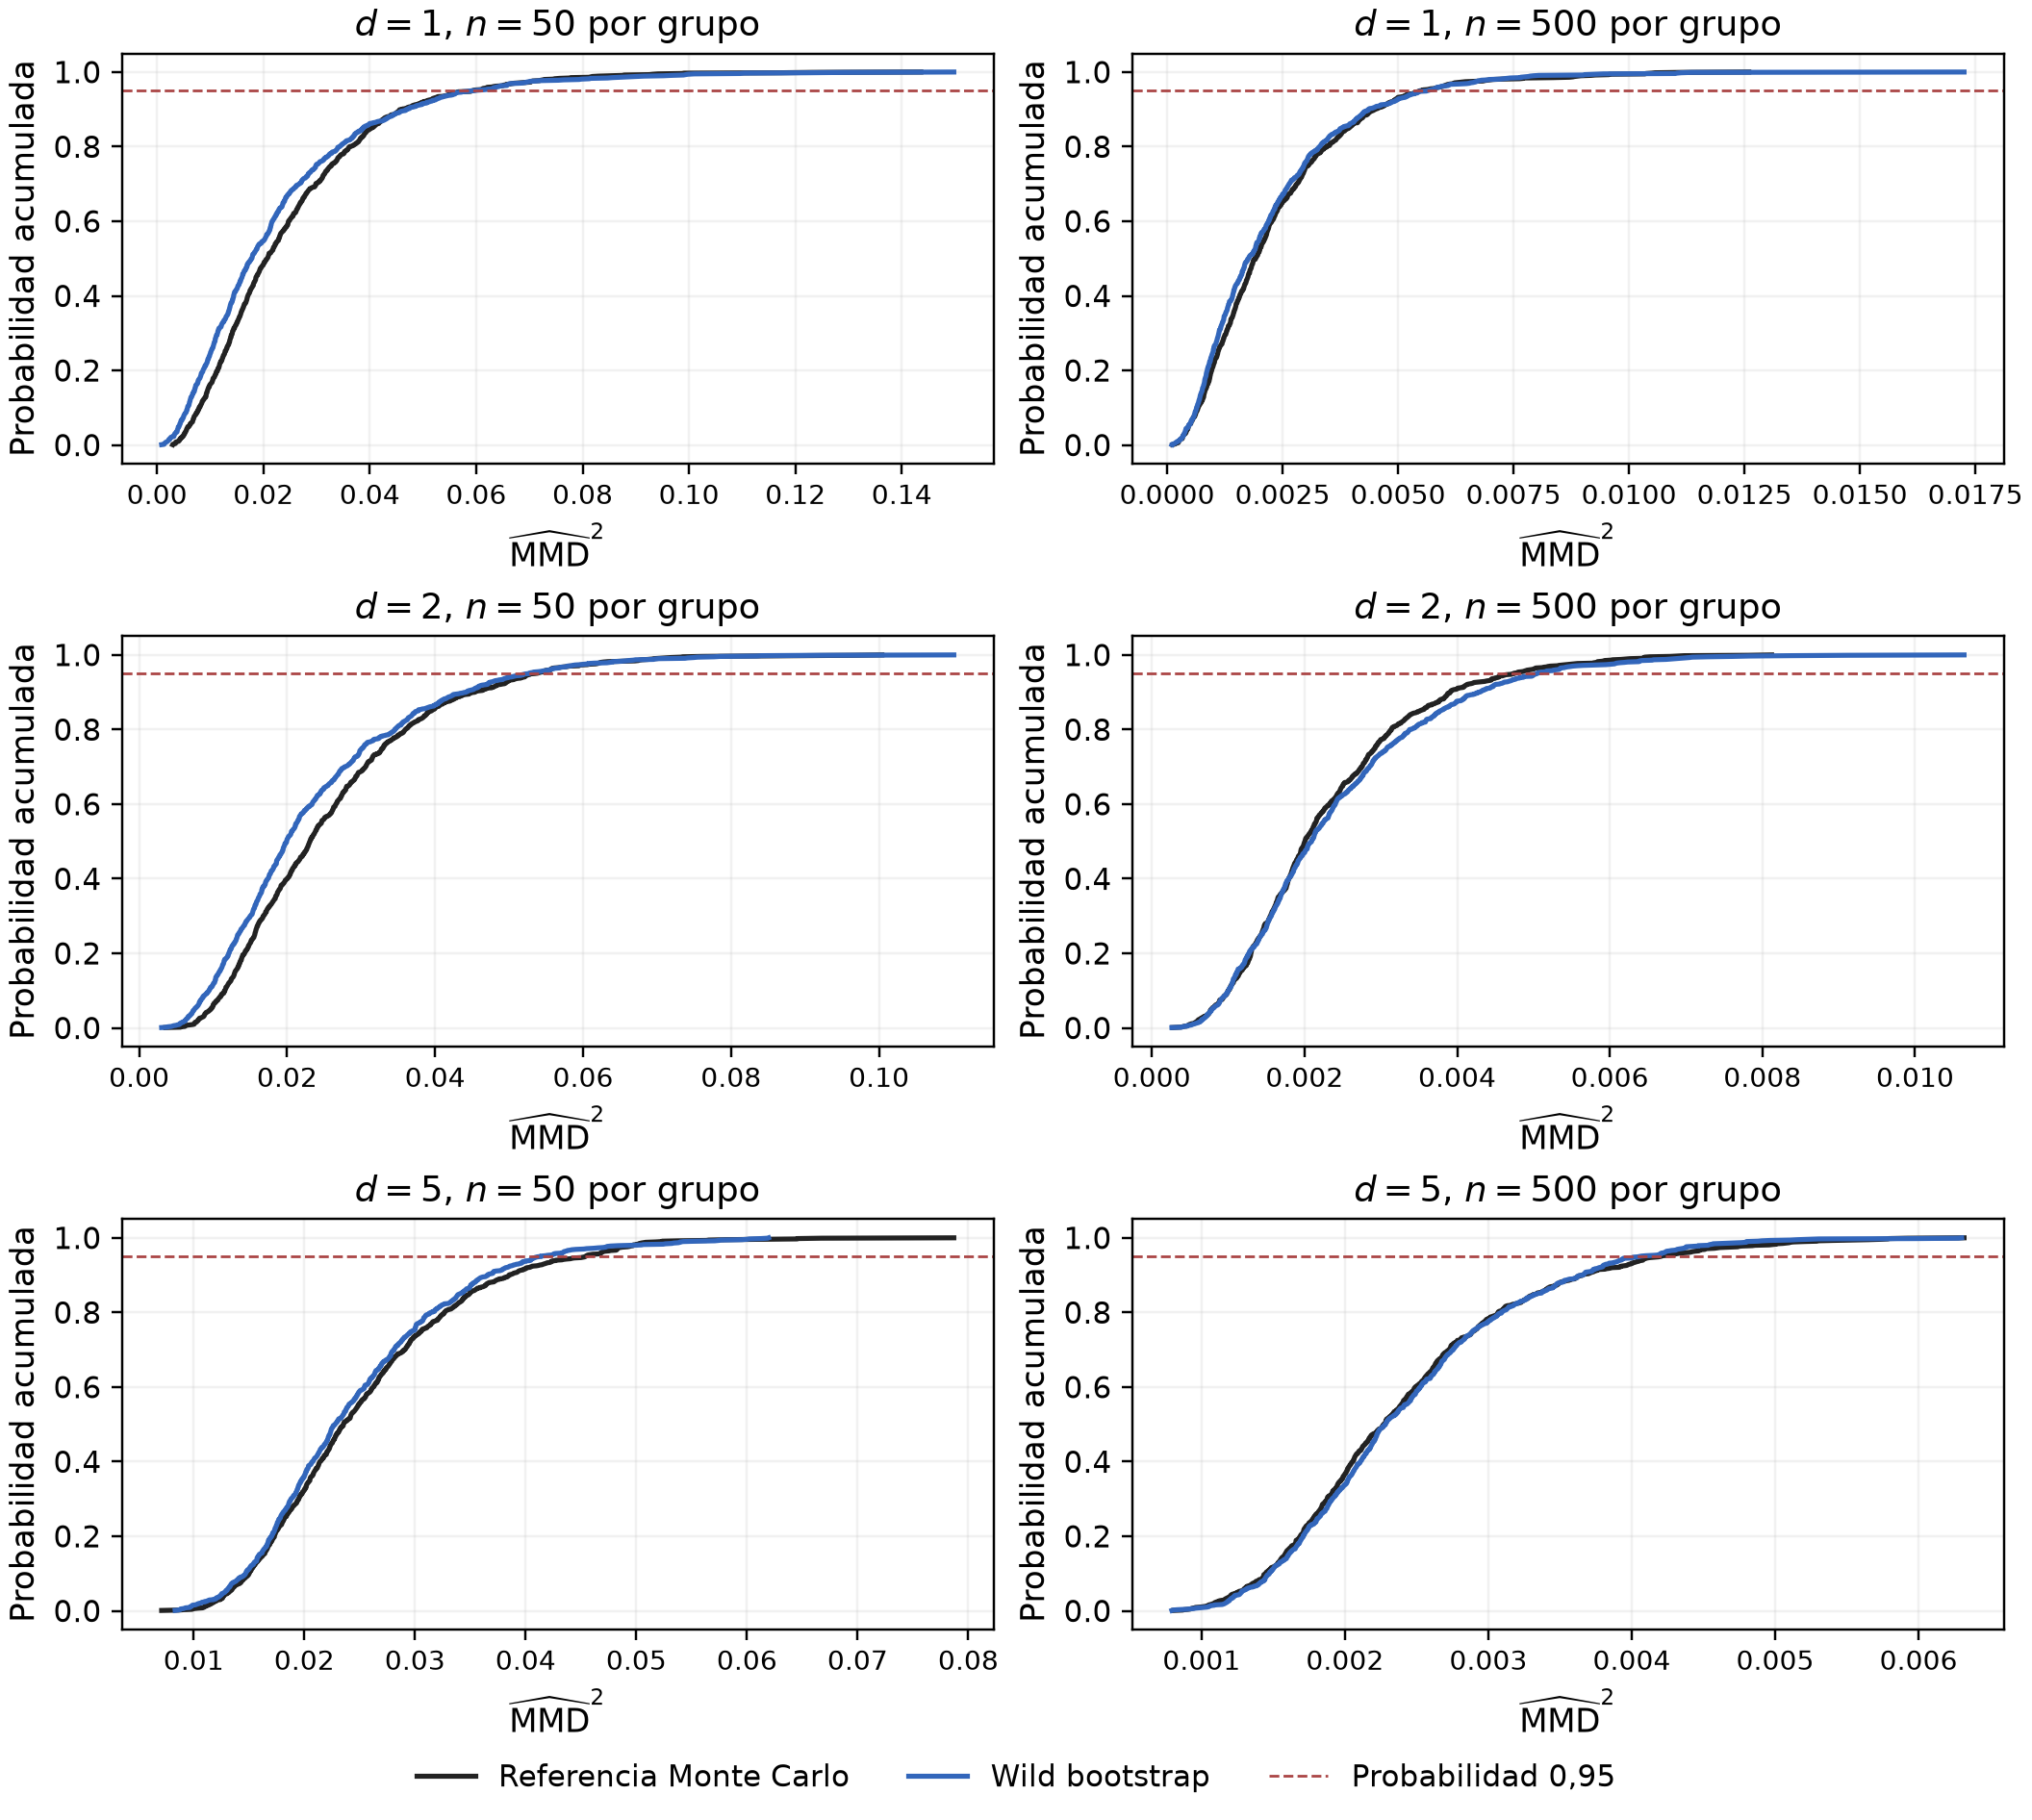
\includegraphics[width=\linewidth]{figuras/cdf_multivariado.png}
\caption{Comparación de la referencia Monte Carlo y el wild bootstrap bajo $H_0:P=Q=\mathcal N_d(0,I_d)$. Filas: $d=1,2,5$; columnas: $n=50,500$. Cada curva contiene 1000 valores. Los ejes horizontales tienen escalas propias para permitir la lectura de cada escenario.}
\label{fig:cdf}
\end{figure}
\clearpage

\section{Alcance y siguientes etapas}
La implementación se ha evaluado en seis configuraciones normales i.i.d., incluyendo observaciones escalares y vectoriales. El kernel continúa produciendo una matriz de similitudes entre observaciones y el WB utiliza un peso por fila; el cambio de dimensión no exige cambiar la fórmula del estadístico. Sin embargo, conservar el algoritmo no garantiza conservar su precisión en muestras finitas.

El siguiente control consiste en repetir cada escenario con distintas parejas iniciales y semillas. Esto permitiría distinguir discrepancias sistemáticas de variabilidad muestral. Si cambia el ancho de banda, cada bootstrap debe compararse con una referencia compatible con ese kernel; alternativamente, puede fijarse un único ancho de banda para todo el conjunto de repeticiones de un escenario. También conviene estimar la incertidumbre de los percentiles antes de interpretar diferencias pequeñas.

El diseño actual emplea covarianza identidad. Una extensión posterior puede introducir correlación entre coordenadas, conservando la independencia entre observaciones. Esto es diferente de incorporar dependencia temporal entre filas. Además, evaluar $d=1,2,5$ no establece una garantía para cualquier dimensión ni para otras familias de distribuciones.

La etapa temporal requiere precisar qué dependencia se introduce y qué estadístico se desea aproximar. La literatura sobre wild bootstrap para tests con kernels ofrece un marco para procesos dependientes \cite{chwialkowski2014}, pero los resultados i.i.d. no se transfieren automáticamente a ese caso. La comparación con Xiao--Lima y el monitoreo de cambios en series quedan fuera de los resultados de este documento.

\section{Conclusiones}
Se extendió la validación de MMD$^2$ y wild bootstrap desde observaciones univariadas a datos en $\R^2$ y $\R^5$, utilizando $n=50$ y $n=500$ por grupo. En todos los casos se aplicó el mismo algoritmo y se comparó su distribución empírica con una referencia Monte Carlo bajo la hipótesis nula.

Los resultados muestran que la precisión varía entre configuraciones. El mayor error absoluto del percentil 95 fue $8{,}87\%$, correspondiente a $n=50$, $d=5$; con $n=500$, el mayor fue $6{,}39\%$, en $d=2$. La comparación multivariada aporta así información que no podía deducirse del caso univariado: el procedimiento se extiende de manera directa, pero su aproximación debe evaluarse en cada escenario.

Estos resultados constituyen evidencia empírica inicial, no una demostración general de convergencia o calibración. El paso siguiente es repetir las configuraciones con nuevas parejas iniciales para evaluar la estabilidad de las discrepancias observadas.

\clearpage
\bibliographystyle{plain}
\bibliography{referencias}

\clearpage
\appendix
\section{Detalles complementarios de la simulación}\label{anexo:detalles}
La Tabla~\ref{tab:complementaria} registra el ancho de banda y las medias empíricas de cada escenario. La regla para seleccionar $\ell$ es la misma, pero su valor crece entre las dimensiones estudiadas porque las distancias entre vectores cambian. El parámetro se mantiene fijo dentro de cada comparación.

\begin{table}[htbp]
\centering
\begin{tabular}{rrrrr}
\toprule
$n$ & $d$ & $\ell$ & Media MC & Media WB\\
\midrule
50 & 1 & 0,54072 & 0,02504 & 0,02302 \\
50 & 2 & 1,04111 & 0,02605 & 0,02385 \\
50 & 5 & 2,00346 & 0,02549 & 0,02464 \\
500 & 1 & 0,66278 & 0,00234 & 0,00224 \\
500 & 2 & 1,17223 & 0,00230 & 0,00242 \\
500 & 5 & 2,08840 & 0,00243 & 0,00244 \\
\bottomrule
\end{tabular}

\caption{Anchos de banda y medias de las distribuciones empíricas. Se utiliza una pareja inicial distinta para cada configuración, generada al reiniciar la semilla 42.}
\label{tab:complementaria}
\end{table}

La Figura~\ref{fig:hist} complementa las CDF del cuerpo principal. Los intervalos del histograma son compartidos por ambas distribuciones dentro de cada panel; las escalas entre paneles pueden diferir. Estos gráficos describen las corridas realizadas y no sustituyen una evaluación sobre múltiples parejas iniciales.

\begin{figure}[htbp]
\centering
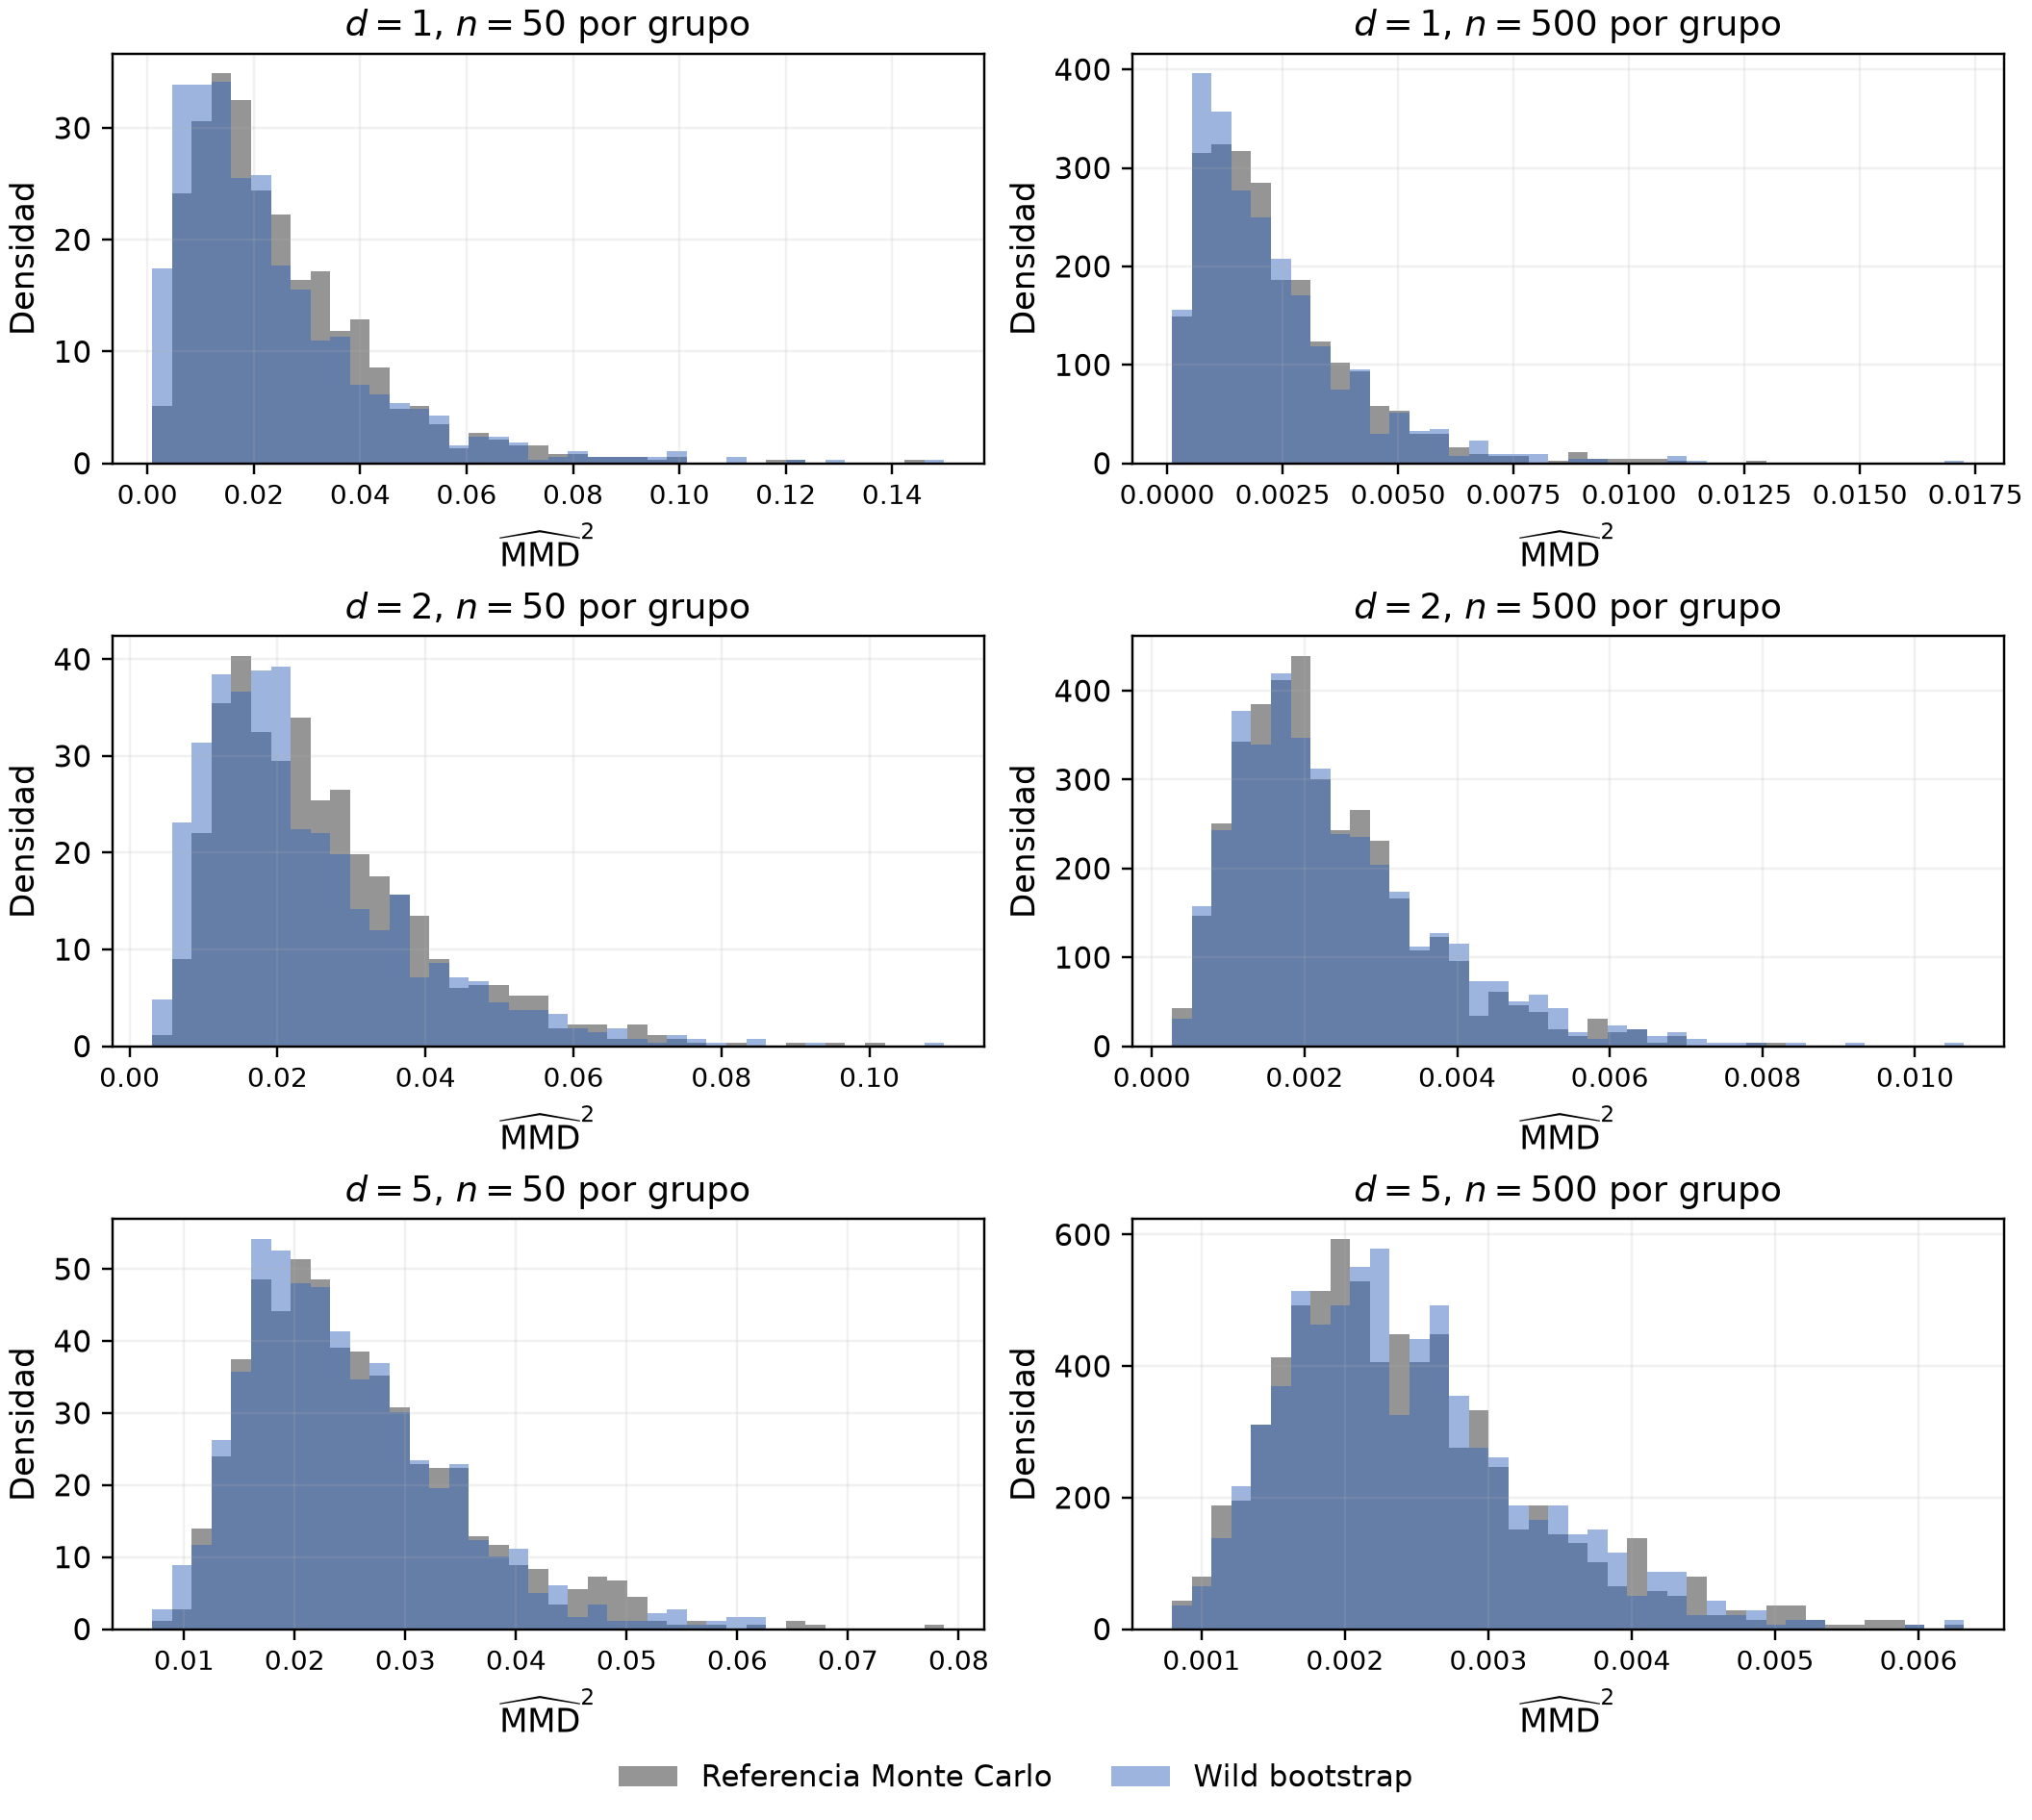
\includegraphics[width=0.93\linewidth]{figuras/histogramas_multivariado.png}
\caption{Histogramas de densidad para las seis configuraciones. El orden coincide con el de la Figura~\ref{fig:cdf}: dimensiones por fila y tamaños por columna.}
\label{fig:hist}
\end{figure}

\end{document}
